33. Раз прямые параллельны, $k=2.$ Подставим координаты точки $A:\ 7=2\cdot2+b,\ b=3.$ Укажем три принадлежащие графику $y=2x+3$ точки: $(-3;-3),\ (-1;1)$ и $(0;3).$
$$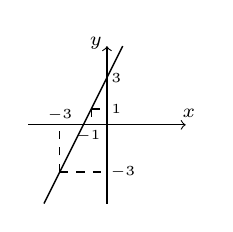
\begin{tikzpicture}[scale=0.2]
\tikzset {line01/.style={line width =0.5pt}}
\tikzset{line02/.style={line width =1pt}}
\tikzset{line03/.style={dashed,line width =0.5pt}}
%\filldraw [black] (0,0) circle (1pt);
\draw [->] (-5,0) -- (5,0);
\draw [->] (0,-5) -- (0,5);
\draw[line01] (-4,-5) -- (1,5);
\draw[line03] (-1,1) -- (-1,0);
\draw[line03] (-1,1) -- (0,1);
\draw[line03] (-3,-3) -- (-3,0);
\draw[line03] (-3,-3) -- (0,-3);
%\draw[line01] (0,-3) -- (-2,5);
\draw (0.6,3) node {\tiny $3$};
\draw (1,-3) node {\tiny $-3$};
\draw (-3,0.6) node {\tiny $-3$};
\draw (-1.2,-0.7) node {\tiny $-1$};
\draw (5.2,0.7) node {\scriptsize $x$};
\draw (0.6,1) node {\tiny $1$};
\draw (-0.7,5.2) node {\scriptsize $y$};
\end{tikzpicture}$$
